\section{Recherche Timo}
\subsection{How robust is the United Kingdom justice system against the advance of deepfake audio and video}
Dieses Paper untersucht, wie geschützt das Rechtssystem in UK vor Deepfakes ist.
Dabei werden Schwierigkeiten bei der Erkennung und vorbeugende Maßnahmen diskutiert.
Das Paper grenzt den Begriff Fakes von Deepfakes, wobei Fakes rein von menschlicher Hand, Deepfakes aber durch den Machine Learning Process erstellt werden.
Zur Vorbeugung nennt das Paper die Schulung und Sensibilsierung von Verantwortlichen in Gerichten zur einfacheren Erkennung von Deepfakes.
Gerade der Einsatz und die Schulung von technischen Forensikern wird empfohlen.
Zur Zeit gibt es noch keinen gesetzlichen Standard bzgl. Deepfakes in UK.\cite{Jones2022}

\subsection{Do (Microtargeted) Deepfakes Have Real Effects on Political Attitudes}
Umfrage mit 278 Teilnehmern, 5 Sekunden deepfaked an Video von Hollänischem Politiker christlicher Partei.
Studie zeigt dass es möglich ist zu manipulieren mit so einem Skandal. 
Das Ansehen sinkt aber eher an den Politker als an seine Partei, dahingehend gibt es nur kleine Auswirkungen.
Ergebnis zeigt dass Deepfakes einen höheren Einfluss haben als die Verbreitung von einfachen Falschmeldungen.
Nur 12 der Teilnehmer erkannten den Deepfake.\cite{Dobber2020}

\subsection{Human Perception of Audio Deepfakes}
Studie Über Erkennung von Audio Deepfakes von 410 Teilnehmern mit Hilfe eines Spiels, indem die Teilnehmer Stimmen hörten und diese als entweder Wahr oder Falsch deklarierten.
Muttersprachler höhere Erkennungschance als Nicht-Muttersprachler.
Ältere Menschen anfälliger als Junge Menschen.
IT-Kenntnis nicht von Bedeutung beim Erkennen von Deepfakes.
Aussicht ist dass die Technologie sich stark verbessern wird, die menschlichen Fähigkeiten zur Erkennung allerdings stagnieren.
Fazit. es braucht technische Erkennung. \cite{Mueller2022}

\subsection{A Review of Image Processing Techniques for Deepfakes}
Deepfakes erreichen Millionen Menschen innerhalb von Sekunden auf Social Image; Gefährlich.
Jeder kann Ziel eines Deepfake-Angriffs sein.
Ergebnis von Studien zeigt, dass man zur Bekämpfung dieser Berdohung die folgenden Maßnahmen ergriffen werden sollten:
Politische Richtlinien, Schulung und Bildung.
Jeder kann mit freier Software Deepfakes erstellen, kein besonderes Wissen nötig (z.B. Faceswap-Apps).
Paper untersucht verschiedene Ansätze von Erkennungen (BILD).
\begin{figure}[h]
 \centering
 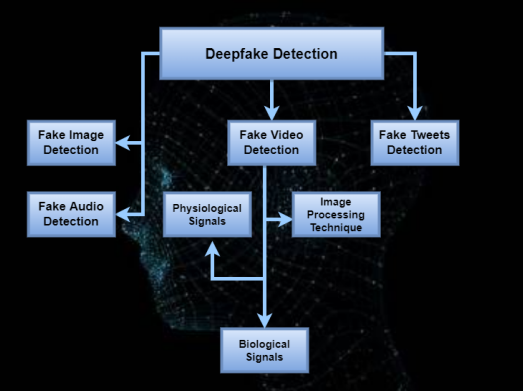
\includegraphics{Assets/DeepfakeDetections.png}
 \caption{Deepfake Detections}
 \label{fig:DeepfakeDetections}
\end{figure}
Unterscheidung zwischen Video, Audio und Tweet-Deepfakes.
Indikatoren zur Erkennung können sein: Kopfhaltung, Anzahl und Dauer von Blinzeln, Hinweise bei der Zahnplatzierung und weitere Gesichtszüge.
Voraussage: Deepfake wird immer weiter Verbreitung finden, vorallem auf Social Media.
\cite{Shahzad2022}

\subsection{FBI Warns That Scammers Are Using Deepfakes to Apply for Sensitive Jobs}
Gestohlene Identitäten für Jobinterviews für Remote-Arbeit mit Hilfe von Audio-Deepfake.
Als Gegenmaßnahme Schulungen für Mitarbeiter zur leichteren Erkennung.
Genutzt um Zugang zu Firmennetzen und Firmendaten zu erhalten.
Dabei sollte man auf die Synchronisation von Lippe und Stimme achten, oft nicht zu 100 Prozent übereinstimmend
Zur Vorbeugung Deepfake Risk Management einführen.
WIE ZITIEREN?